\documentclass[12pt]{article}%
\usepackage{amsmath}%

%\usepackage{bibentry}%
\usepackage{amsfonts}%
\usepackage{amssymb}%
\usepackage{setspace}%
\usepackage{bbm}%
%\usepackage{harvard}
%\usepackage{chicago}
%\bibpunct[,~]{(}{)}{;}{a}{}{,}
\usepackage{enumerate}%
\usepackage{xfrac}
\usepackage[top=1in, bottom=1in, left=1in, right=1in]{geometry}
\usepackage{multirow}
\usepackage{rotating,graphicx}
\usepackage{subcaption}
\usepackage{caption}
\usepackage{rotating}
\usepackage{booktabs}
\usepackage[flushleft]{threeparttable}
\usepackage{subcaption}
\usepackage{float}
\usepackage{appendix}
\usepackage{titletoc}


\usepackage[bookmarks=false,colorlinks=true, linkcolor=black, urlcolor=black, citecolor=black]{hyperref}

\usepackage{fullpage}

\usepackage{titlesec}

\usepackage[comma,longnamesfirst]{natbib}%

\newtheorem{hypothesis}{Hypothesis}
\usepackage{xcolor}

\usepackage{xr}

\pdfminorversion=6
\bibpunct[,~]{(}{)}{;}{a}{}{,}
\bibliographystyle{apsr}



\author{Sarah ``Dot" Warren\thanks{Ph.D. student, University of Rochester. Harkness Hall, 333 Hutchinson Rd, Rochester, NY 14627. swarr15@ur.rochester.edu.}}
\title{Who Benefits? Experimental Evidence of Gender Differences in Aid Allocations\thanks{The experiment reported in this paper is preregistered at EGAP Registry (https://osf.io/u5wxg/). This research was reviewed and approved by the Florida State University Institutional Review Board. All errors remain the author's own responsibility.}}


\date{PRELIMINARY DRAFT - PLEASE DO NOT CIRCULATE}

\begin{document}
\maketitle
\thispagestyle{empty}


\begin{abstract}
While past work clearly demonstrates that women are rewarded less compared to men in the labor market, how do they fare when taking up government aid? Some literature suggests that women taking up aid will continue to be evaluated unfairly, because they are not perceived as having equal income-potential to men; other work suggests that benevolent sexist attitudes may disproportionately reward female applicants relative to similarly-situated men. Given the competing intuitions behind rewarding or punishing men seeking welfare, an experimental test of each hypothesis is presented. I find that, on average, male applicants earn less than female applicants with identical needs. Further, I find the amount awarded to women varies conditional on being rated a ``Poor” or ``Excellent” worker by a third party, while there is no difference in the amount awarded to men who are rated ``Poor” workers compared to men who are rated ``Excellent” workers. Thus, women’s advantage over men applicants extends only so far as women are perceived as ``deserving.” The totality of these results suggest that people are more inclined to help poor women rather than poor men, but only deserving women, when the quality of women applicants is validated by an external source. I bolster these findings with preliminary analyses suggesting that near-identical trends hold across respondent ideologies. %this abstract is bad and I have no intention of fixing it. 213 words
\end{abstract}
%\vspace{0.5cm}


\newpage


\pagenumbering{arabic}
\begin{doublespace}

Across many policy areas, including Medicaid \citep{weissert1994beyond}, labor \citep{schmidt2002politicization}, disability insurance \citep{keiser1999state}, welfare \citep{kogan_welfare_2021}, and immigration \citep{lewis2013some}, street-level bureaucrats use their discretion to align realized policy outcomes with personal and community values, even when their formal responsibility is to implement otherwise identical statutory language. While this bureaucratic discretion may lead to higher responsiveness in some cases, it opens the door for unequal treatment of potential beneficiaries. This is problematic, because the task of the bureaucrat is to neutrally apply the law. Yet despite the well-documented reality that welfare attitudes are racialized \citep{desante_working_2013, gilliam_welfare_1999}, the question of whether welfare attitudes are conditioned by gender has received limited attention. Indeed, much of the work on welfare attitudes uses exclusively female names or images, limiting scholars' ability to draw inferences about the ways gender might interact with individuals welfare attitudes \citep{desante_working_2013, winter_beyond_2006, gilliam_welfare_1999, goren_pliable_2022}. Bureaucratic discretion may allow individuals to respond differently to a woman in need than a similarly situated man in need, even if their objective economic needs are identical.  Understanding the relationship between bureaucratic discretion and taste-based discrimination against women is therefore of paramount importance to scholars of bureaucratic politics and democratic responsiveness.

The present study enters the debate about modern sexism, American values, and bureaucratic responsiveness to show that, when men and women are put in direct competition for scarce public resources, gender-based prejudice interacts with American perceptions of work ethic to amplify existing, harmful stereotypes about men and women. I find that, on average, male applicants earn less than female applicants with identical needs. Further, I find the amount awarded to women varies conditional on being rated a ``Poor” or ``Excellent” worker by a third party, while there is no difference in the amount awarded to men who are rated ``Poor” workers compared to men who are rated ``Excellent” workers. Thus, women’s advantage over men applicants extends only so far as women are perceived as ``deserving.” The totality of these results suggest that people are more inclined to help poor women rather than poor men, but only deserving women, when the quality of women applicants is validated by an external source. This research provides evidence toward benevolent sexism, in which women are viewed as weak and in need of extra care \citep{glick_hostile_1997, glick_ambivalent_2001}. It additionally informs our understanding of gender differences in considerations of the deserving poor and the consequences of these considerations on bureaucratic responsiveness.

The rest of this paper proceeds as follows...

\section*{Theory and Hypotheses}
Sexism toward women may be hostile or benevolent; while both forms of sexism share the assumption that women are inferior to men and restrict women to a lower social status, they manifest in different behavior patterns. Hostile sexism constitutes punitive behavior toward women who deviate from their prescribed role as heterosexual domestic laborers, whereas benevolent sexism manifests in protective coddling of women who stay within this role. Benevolent sexism reflects evaluations of women that are seemingly positive, but remain caustic to gender equity and restrict women's personal, professional, political, and social opportunities. Examples of benevolently sexist attitudes include the reverence of women exclusively in wife, mother, and child-caretaker roles, the romanticizing of women as objects of heterosexual affection, and the belief that men have a strict duty to protect women \citep{chen_gender_2020, geus_understanding_2022}. Failing to remain within the confines of these traditional roles may trigger punishment in the form of hostile sexism. Examples of hostile sexism include beliefs about women as incompetent, unintelligent, overly emotional, and sexually manipulative \citep{mcthomas_growing_2016, cassese_playing_2019}.

How should we expect these attitudes to manifest when evaluating welfare applicants? While we have long known that women experience discrimination in ways men do not, there remains uncertainty about whether norms of male favoritism should carry into welfare outcomes. Women receive different treatment in everything from applying to jobs \citep{quadlin_market} to running for office \citep{hassell_partys_2019} to the price they pay for basic household goods in some countries \citep{betz_womens_2021}. Economically, women earn less than their male counterparts \citep{mandel_up_2013}. However, the vast literature documenting the more favorable treatment of men relative to women primarily concerns traditionally masculine domains: salary negotiations \citep{castillo_gender_2013}, hiring decisions \citep{neumark_sex_1996, goldin_orchestrating_2000}, and elections \citep{clayton_how_2020}. In these environments, the dimensions on which participants are being evaluated are frequently perceived as masculine qualities, incongruent with traditional feminine presentation \citep{eagly_role_2002, koenig_are_2011}. Insofar as these norms carry into welfare allotments, they suggest that we should expect men to be favored when applying for aid, since they may be viewed as inherently possessing better odds of succeeding once back into the labor force.

In contrast, the task of the bureaucrat is to evaluate applicants neutrally on the basis of their economic needs and eligibility for the specific program for which they are applying. Public aid is designed to be an environment in which gendered personal characteristics should be irrelevant. If this is truly the case, then we may expect that norms of male favoritism may not hold here. Further, welfare is distinct from labor market domains in that it carries with it social stigma \citep{soss_lessons_1999} and negative stereotypes \citep{foster_welfare_2008, esping-andersen_welfare_2015}. Unlike in the labor market, where men continue to out-earn their female counterparts, women are more likely than men to benefit from public aid \citep{fraser_women_1989, lundberg-love_women_2012, abramovitz_regulating_2017}.


While it is possible that norms of male favoritism could persist, I argue that it is more likely that women applying for aid will activate benevolently sexist attitudes. That is, women applying for aid will be seen as needier and more deserving than identically-situated male applicants because she is perceived as needing protection. Compounding this, Americans have long believed people ``ought to take care of their personal problems by themselves” without relying on the government for aid \citep{sniderman_coping_1977}. The feminization of welfare, combined with the perceived failure of men seeking public assistance to achieve the masculine ideal of breadwinning, may contribute to a hostility for men receiving public benefits: such policies help those who should be helping themselves \citep{bobocel_justice-based_1998, katz_racial_1988, sniderman_symbolic_1986, sniderman_beyond_1996, mclosky_ethos}. Building on this body of work, I hypothesize that male aid applicants will be awarded less than female applicants.

\begin{hypothesis} \label{hyp:first}
	On average, male applicants will be awarded less than female applicants.
\end{hypothesis}

\subsection*{Deservingness: Competence and Quality}
Another dimension that has characterized past work and public debate on welfare is deservingness \citep{schneider_social_1993, van2017social, gilens_why_2000}. The ``deserving poor” are those whose personal financial circumstances have been devastated by structural or macroeconomic forces beyond the individual’s control, rather than personal qualities of dependence and laziness \citep{van_oorschot_who_nodate}. Thus, conditional on gender, an individual’s deservingness should also affect the amount of aid they are awarded. Because notions of deservingness and undeservingness are frequently characterized by ability and willingness to work, we might think that factors like individual competence will affect aid allocations. Specifically, high competence workers should receive more than their low-competence counterparts.


\begin{hypothesis} \label{hyp:second}
On average, high-competence applicants will be awarded more than low-competence applicants.
\end{hypothesis}


Deservingness might also be signaled by an external evaluation of worker-quality. If individuals truly prioritize giving aid to good workers whose personal financial circumstances were devastated by forces outside of their control, then high-quality workers should be awarded more than low-quality workers. However, evidence suggests that external or objective proof of women’s capabilities may be valuable resources in offsetting negative perceptions of women as workers, but offer minimal or no returns for men \citep{abel_value_2020, dadgar_labor_2015, jepsen_labor-market_2014}. I therefore hypothesize:


\begin{hypothesis} \label{hyp:thirda}
	For male applicants, there will be no significant difference between amounts awarded to ``Excellent” workers as compared to ``Poor” workers.
\end{hypothesis}

\begin{hypothesis} \label{hyp:thirdb}
	For female applicants, there will be a significant difference between amounts awarded to ``Excellent” workers as compared to ``Poor” workers.
\end{hypothesis}


\section*{Experimental Design and Data}
To test how gender, worker quality, and perceived work ethic shape attitudes toward welfare recipients and the amounts they are awarded, I conducted a survey experiment in which participants were asked to budget money to different pairs of applicants for state assistance. Following DeSante (2013), I use hand-redacted welfare applications to manipulate targets’ for assistance sex, perceived competence, and objective work-quality rating (Figure \ref{characteristics}).

To manipulate objective quality, each applicant is randomly assigned a rating of ``Excellent” or ``Poor." To manipulate sex and perceived competence, I use two male and two female names from Hayes and Mitchell’s (2020) name-characteristics dataset: Sandra, James, Misty, and Sammie.\footnote{To create the dataset, the authors obtained a list of given names among people born in the United States between the years 1955 and 1990 from the U.S. Social Security Administration (SSA). To identify the gender of the names, they used information on sex included in the SSA data.} These names were specifically selected to minimize the likelihood that factors other than sex, objective, and perceived work ethic would affect treatment. Names are used rather than more overt cues to minimize demand effects \citep{quidt_experimenter_2019}. To mitigate concerns about the effects of race and the racialization of welfare confounding results, all four names chosen were coded as racially distinct white names in the \cite{hayes_2020} names dataset. These names are matched on characteristics that Americans report as relevant considerations when considering welfare support \citep{bobocel_justice-based_1998, katz_racial_1988, sniderman_symbolic_1986, sniderman_beyond_1996, mclosky_ethos}. Sandra and James are rated highly in professionalism, competence, and work ethic, while Sammie and Misty are rated lower in all three characteristics. All names are comparable in estimates of whiteness, honesty, and likeability. Figure \ref{characteristics} below shows the complete breakdown of name-characteristics.

%%NAME CHARACTERISTICS FIGURE HERE
\begin{figure}[h!]
	\centering
	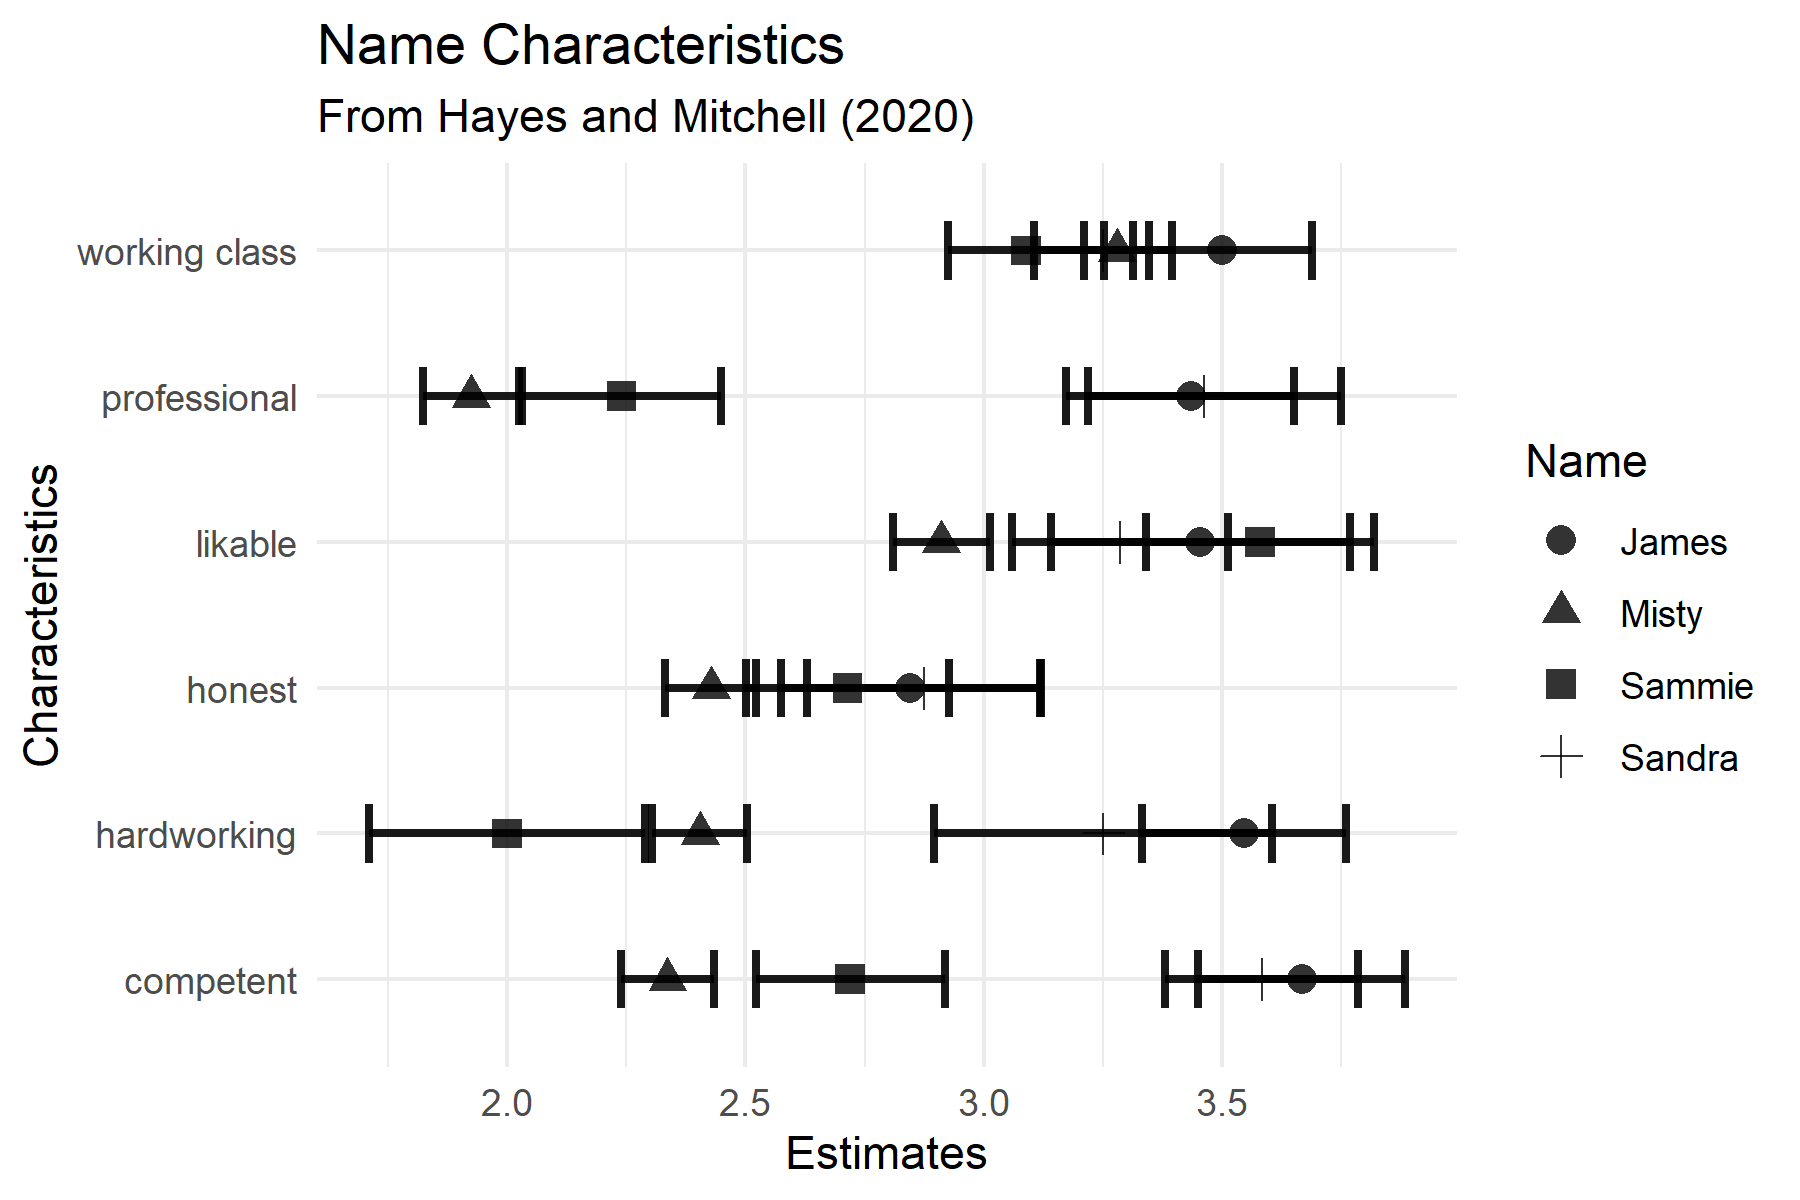
\includegraphics[scale=1]{figs/characteristics.png}
	{\singlespacing
		\parbox{0.78\textwidth}{\scriptsize%\vspace{-0.25cm}
			Notes: Explain the figure here
	}}
	\caption{Differences in Valence Characteristics Between Treatment Names}
	\label{characteristics}
\end{figure}


Subjects are given a budgeting task in which they are asked to allocate \$1,500 to two applicants for federal assistance, each of whom has a state-determined need of \$900. Respondents may also choose to give some or all of the funds to ``offset the state deficit.”  Participants were given significant discretion in how aid was awarded, constrained only by a budgetary constraint and the inability to give an applicant more than their assessed need. Given the budget constraint—both applicants’ full need cannot be met—I use the amount awarded to Applicant 1, Applicant 2, and the Government as a direct estimate of an applicant’s deservingness. These allocations are my main variables of interest. Everything else about the applicants remains identical, except for a worker quality assessment of Excellent or Poor and their name, which cues both sex (male or female) and competence (high or low). Given this, if an applicant receives a different allocation across treatments, we can infer that this difference is due to experimental manipulation. As the applicant’s characteristics were manipulated via random assignment, any difference in the relative importance respondents place on fiscal responsibility—illustrated by giving more to offset the budget deficit—can also be traced back to the experimental treatment. This deficit option also allows for individuals to take a principled position, a socially desirable and available option, to decide that the money would be better spent in some other way.

%%SAMPLE APPLICATIONS FIGURE HERE
\begin{figure}[h!]
	\centering
	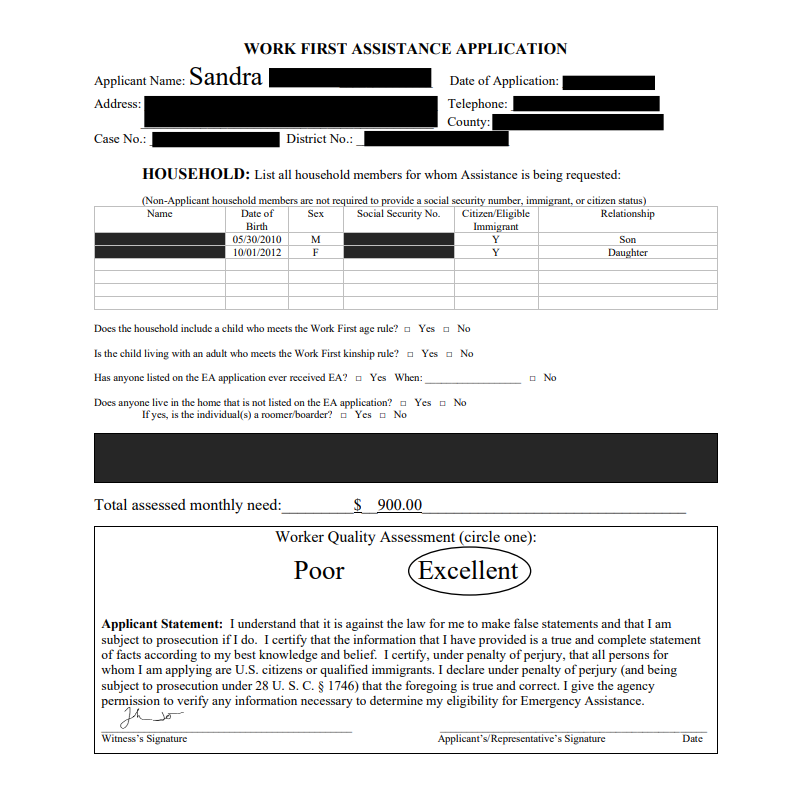
\includegraphics[scale=1]{figs/example_treatment.png}
	\caption{Example Aid Application}
	\label{figure2}
\end{figure}


In order to isolate the effects of sex versus the traits people ascribe to different names, I fielded a survey experiment with YouGov (n=2150) in April 2022. Modeled after \cite{desante_working_2013}, respondents viewed two applications identical in appearance to the original experiment. Rather than randomizing both applications, all respondents viewed the same baseline application of ``Sandra” who was rated as ``Excellent” compared to a second application. I used a 2x2x2 factorial design for this second application, randomizing sex (male/female), competence (high/low), and quality assessment (excellent/poor) of the second application, using the names James, Misty, and Sammie as my cue for sex and competence. Respondents were then asked to allocate funding to the two applicants or to offset the state budgetary deficit.

\section*{Experimental Results}
When men and women are put in direct competition for scarce resources, how do women fare compared to similarly-situated men? How does perceived competence and external quality ratings affect this relationship? Figure \ref{results-main} presents the main results of the experiment by treatment name, with color denoting the quality rating (Excellent/Poor) of the treatment name, and point-shape denoting the amount given to each recipient. Recall that the baseline condition is an applicant named Sandra, a high-competence name, who is rated as an ``Excellent” quality worker.

%%MAIN RESULTS FIG HERE
\begin{figure}[h!]
	\centering
	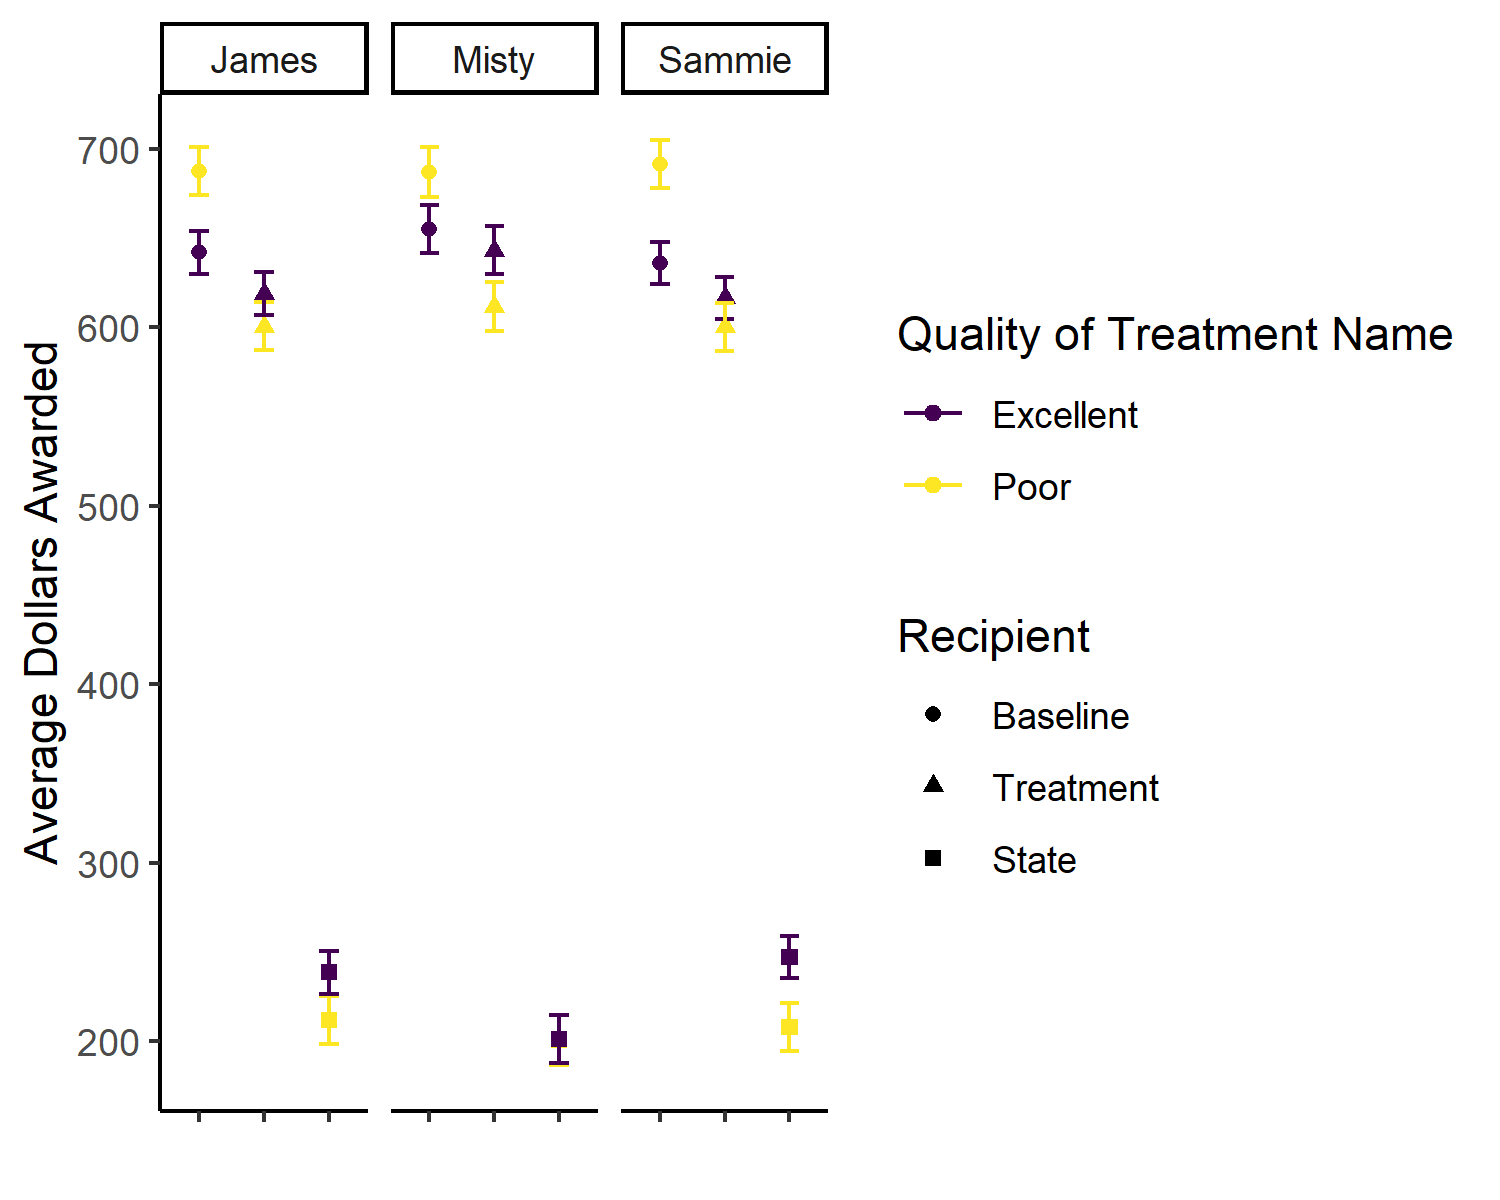
\includegraphics[scale=.8]{figs/general-results-name.png}
	{\singlespacing
		\parbox{0.78\textwidth}{\scriptsize%\vspace{-0.25cm}
			Notes: Explain the figure here
	}}
	\caption{Gender Differences in Aid Allocated by Treatment Name}
	\label{results-main}
\end{figure}

H1 predicts that, on average, male applicants will be awarded less than female applicants. The first panel of Figure \ref{results-main} demonstrates that, when she is paired with a high-competence, ``Excellent” male name, James, Sandra is awarded significantly more on average (\$642.06 vs. \$619.20, p = 0.014). Excellent Sandra also earns more on average than Sammie, a low-competence name, when he is rated ``Excellent” (\$635.98 vs \$616.60, p=0.000). However, there is also no significant difference between Excellent Sandra and Excellent Misty (\$655.31 vs \$643.20, p=0.141). These results are consistent with H1, in that Excellent Misty earns no less than Excellent Sandra, while Excellent James and Excellent Sammie earn substantively and significantly less than the baseline.

Turning to competence, I consider the difference between name valence characteristics and aid amounts awarded. Recall that competence is determined by valence-characteristic scores in the Names Dataset \citep{hayes_2020}. Hayes and Mitchel’s findings suggest that name-characteristics have the potential to minimize differences in aid allotment due to racial prejudice; however, the mitigating effects of name-characteristics do not appear to extend to gender bias. Sandra and James are both high-competence names, while Misty and Sammie are relatively low-competence. I predicted in H2 that high competence names should receive more, on average, than low competence names. Thus, holding applicant quality constant, Sandra should receive more than Misty and James should receive more than Sammie, relative to the baseline. I do not find empirical support for H2. There is no statistically or substantively significant difference between the amounts awarded to Excellent Misty and Excellent Sandra (\$655.31 vs \$643.20, p=0.141), nor is there between Excellent James and Excellent Sammie (\$619.20 and \$616.60, p=0.88), and Poor James and Poor Sammie (\$600.60 and \$600.32, p=0.986). This suggests that, among whites, perceived competence matters less than when making inter-racial comparisons.

Finally, I predicted that, for male applicants, there will be no significant difference between amounts awarded to workers rated ``Excellent” as compared to workers rated ``Poor.” Conversely, I predicted that the opposite will be true for female applicants; that is, worker quality rating will result in a significant difference in the amount awarded. To evaluate H3 and H4, I compare the difference in means for each treatment name to (James, Sammie, and Misty) when they are ``Excellent” rated workers to when they are rated ``Poor.” Table \ref{lasttable} shows the results of this test, which support H3 and H4. There is a statistically significant difference in the amount of aid awarded to Excellent Misty compared to Poor Misty; however, there is no such difference between Excellent Sammie or James compared to Poor Sammie or James.

\begin{table}[]
	\label{lasttable}
	\centering
	\begin{tabular}{lllll}
		\textbf{Treatment Name}      & \textbf{Excellent}            & \textbf{Poor}                 & \textbf{Difference}             & \textbf{p-value}           \\ \hline
		\multicolumn{1}{|l|}{Misty}  & \multicolumn{1}{l|}{\$643.20} & \multicolumn{1}{l|}{\$611.80} & \multicolumn{1}{l|}{\$ - 31.40} & \multicolumn{1}{l|}{0.044**} \\ \hline
		\multicolumn{1}{|l|}{Sammie} & \multicolumn{1}{l|}{\$619.20} & \multicolumn{1}{l|}{\$600.59} & \multicolumn{1}{l|}{\$-18.16}   & \multicolumn{1}{l|}{0.256} \\ \hline
		\multicolumn{1}{|l|}{James}  & \multicolumn{1}{l|}{\$616.60} & \multicolumn{1}{l|}{\$600.32} & \multicolumn{1}{l|}{\$ - 16.28} & \multicolumn{1}{l|}{0.351} \\ \hline
	\end{tabular}
\end{table}


The totality of these results suggest that identically-situated men and women are evaluated differently when put in competition for scarce resources and when bureaucrats enjoy much discretion. Though implicit competence does not appear to play a role in aid evaluations when comparing white men and women to each other, positive third-party quality ratings affect women’s earnings and do not alter men’s. One possible interpretation of this result is that people think of women on average as riskier ``bets” than men. Extra information, like a third-party quality rating, is therefore much more valuable. Whereas, if men are considered relatively safe, stable ``bets,” additional information may have limited impact.

\section*{Implications for Bureaucratic Responsiveness\footnote{Exploratory analysis. The following analysis was not part of my pre-registration plan.}}
Perhaps the most immediate implication of these experimental results is for the federal bureaucracy. If these trends hold among the average member of the bureaucracy, then this suggests that men and women may receive aid at different rates, in part, due solely to their gender. Of course, this is a survey of the general public, not bureaucrats, whom we know differ from the public on relevant dimensions such as liberalism \citep{spenkuch_ideology_2021}, which may mitigate the gender differences I observe in the public. On the other hand, this survey utilizes names as the sole cue of an applicants’ gender, while street-level bureaucrats not only see applicants’ names, but conduct phone interviews with them, have access to their personal financial circumstances, and meet with them in person.

%%FIG OF RESULTS BY IDEOLOGY HERE
\begin{figure}[H]
	\centering
	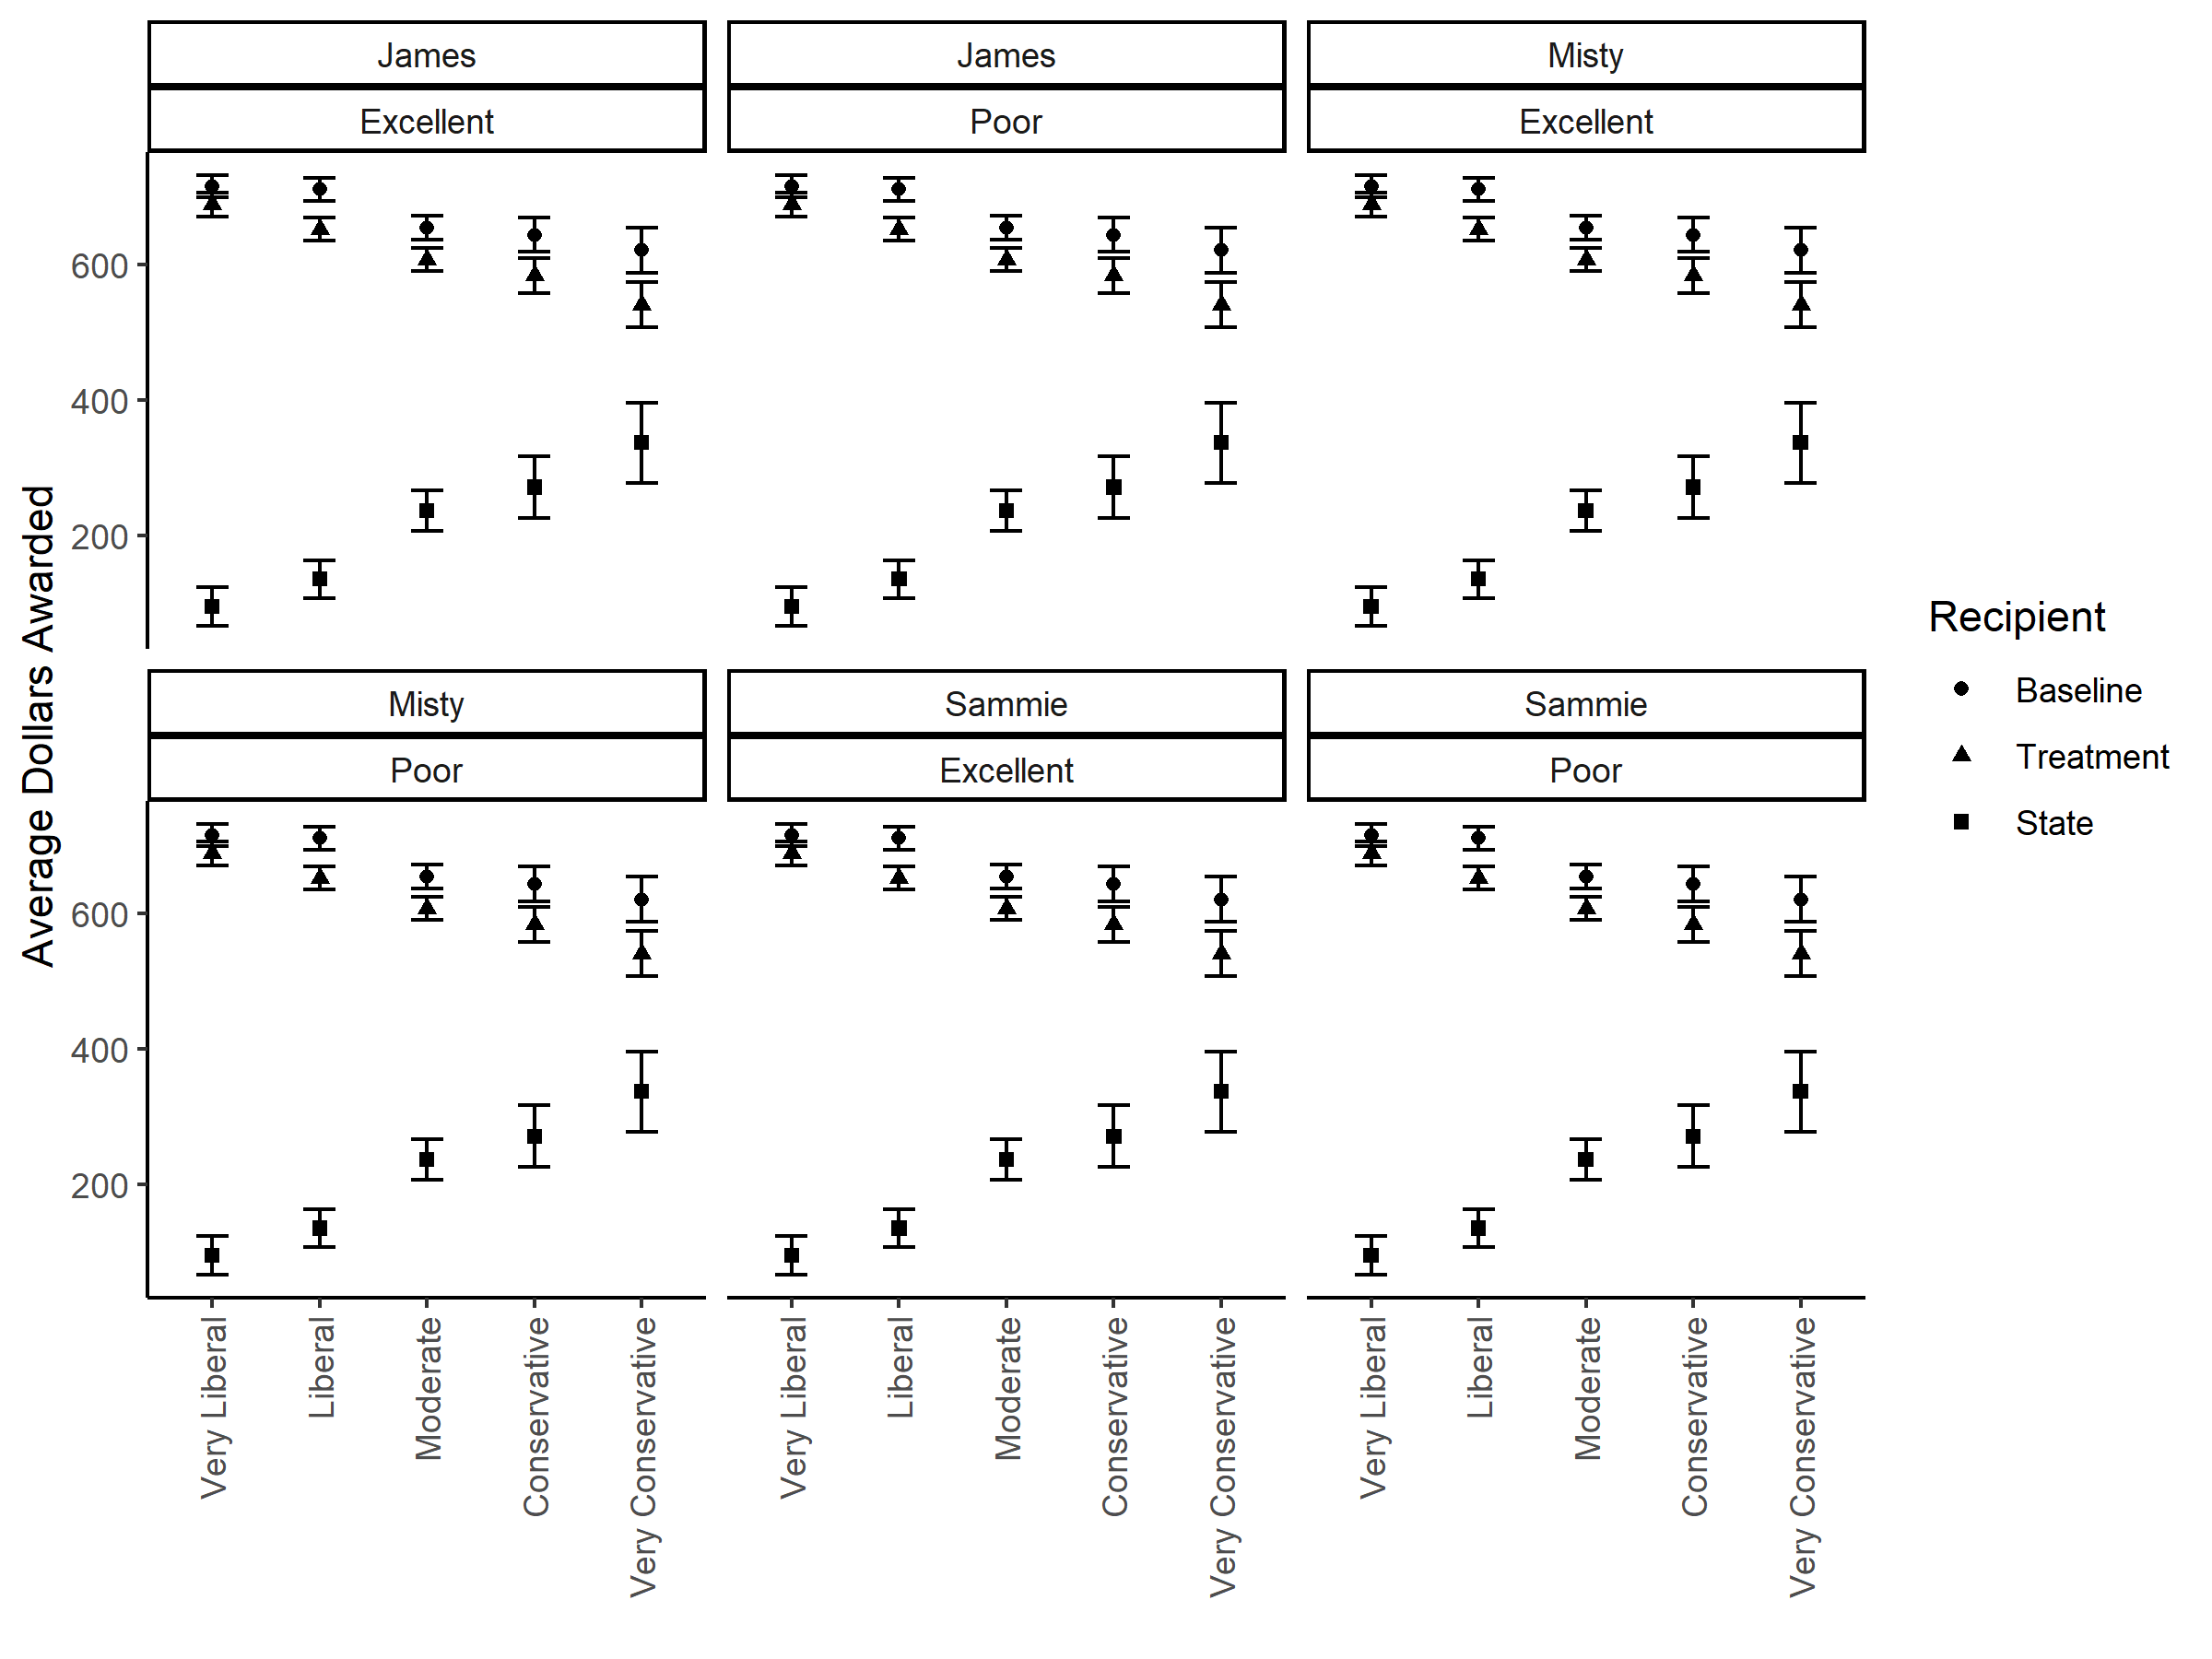
\includegraphics[scale=.8]{figs/robust_result_ideo.png}
	%{\singlespacing
	%	\parbox{0.78\textwidth}{\scriptsize%\vspace{-0.25cm}
	%		Notes: Explain the figure here
	%}}
	\caption{Average Aid Allocations by Ideology}
	\label{ideology}
\end{figure}


While we cannot know from the analysis presented above how bureaucrats would respond if they participated in this experiment, we can break the analysis down by relevant dimensions. Specifically, we can look at differences in allocations by ideology. Figure \ref{ideology} shows the amount given to each recipient for each treatment group broken down by ideology. The more liberal a participant, the more on average they give to applicants and the less they give to the state. However, there remain significant differences in the amounts awarded to respondents that mirror the same trends I found in the aggregated sample. This suggests that, even within liberal environments, these gender disparities may persist.

Notably, as conservatism increases, respondents give less to applicants and more to the state. Indeed, \ref{table} shows that, controlling for each of the possible treatment conditions, for every one unit increase in conservatism on the ideology scale, respondents give approximately $\$44.47$ more to the state.

\begin{table}[!htbp] \centering 
	\caption{} 
	\label{table}
	\begin{tabular}{@{\extracolsep{5pt}}lc} 
		\\[-1.8ex]\hline \\[-1.8ex] 
		\\[-1.8ex] & Dollars Given to State \\ 
		\hline \\[-1.8ex] 
		Ideology & 44.472$^{***}$ \\ 
		& (5.673) \\ 
		Treatment Female & $-$27.835 \\ 
		& (19.926) \\ 
		Rated Excellent & 16.169 \\ 
		& (16.340) \\ 
		High Competence & $-$1.363 \\ 
		& (20.039) \\ 
		Constant & 77.193$^{***}$ \\ 
		& (24.090) \\ 
		N & 1,824 \\ 
		R$^{2}$ & 0.035 \\ 
		Adjusted R$^{2}$ & 0.033 \\ 
		Residual Std. Error & 348.513 (df = 1819) \\ 
		F Statistic & 16.359$^{***}$ (df = 4; 1819) \\ 
		\hline \\[-1.8ex] 
		\multicolumn{2}{l}{$^{*}$p $<$ .1; $^{**}$p $<$ .05; $^{***}$p $<$ .01} \\ 
	\end{tabular} 
\end{table} 

Taken together, these results suggest that, while greater generosity to applicants is associated with liberalism, gender differences in the amount allocated persist across ideologies. Thus, if street level bureaucrats mimic the general public’s behavior in this domain, we may expect these gender differences to persist. Further, more conservative respondents prefer allocating funds to the state irrespective of treatment-level factors like applicant sex, competence, or quality.

\section*{Concluding Discussion} 
Gender and the American value of hard work greatly influence how Americans evaluate the deserving poor. In this survey experiment, I find that both applicant gender and applicant quality effect how ``deserving" the applicant is perceived by respondents. These results show how work ethic matters differently for men and women. While women receive more on average than men, women's perceived deservingness appears to be contingent on their quality-rating, but men's deservingness is not. I bolster these findings by using the data I have to speak to the most immediate implication of these findings: bureaucratic responsiveness. I find that greater generosity to applicants is associated with liberalism, while more conservative respondents prefer to allocate more funds to the state.

\end{doublespace}


\bibliography{womenref}


\end{document}
